\section{Experience}
\label{sec:experience}

In this section, we describe our deployment and operational experience of
\sysname. We build dedicated AI clusters for LLM training. Over the years, we
have iterated several versions of our specialized AI cluster architecture, and
we are currently operating several AI clusters with varying size and hardware
configurations. We use these AI clusters to train a wide range of models, from
computer vision and recommendation models to LLMs. With the increasing
importance of LLMs, we are building AI clusters with larger size to cater the
need of LLM training. As of September 2023, the largest AI cluster in our
production for LLM training contains more than 10,000 NVIDIA Ampere GPUs. We are
also in the process of building large clusters based on the newest NVIDIA Hopper
GPUs, as NVIDIA is ramping up production.


\begin{table}[!t]
    \def\barr{\begin{tabular}{c}}
    \def\earr{\end{tabular}}
    \centering
    \begin{tabular}{c|c|c|c|c|c}
        \hline
         % {\shortstack{Model \\ Size}} & 
         \barr {Model}\\{Size} \earr &
         {Heads} & 
         % {\shortstack{Hidden \\ Size}} & 
         \barr {Hidden}\\{Size} \earr &
         {Layers} & {TP} & {PP}  \\
         \hline
         175B & 128 & 12288 & 96 & 8 & 8 \\
         530B & 160 & 20480 & 105 & 8 & 35 \\
         \hline
    \end{tabular}
    \caption{Model configurations.}
    \label{tab:exp-model-config}
\end{table}


\begin{table*}[ht]
    \centering
    \begin{tabular}{|c|c|c|c|c|c|c|c|}
        \hline
        \multirow{2}{*}{Batch Size} & \multirow{2}{*}{Method} & \multirow{2}{*}{GPUs} & \multirow{2}{*}{\shortstack{Iteration Time (s)}} & \multirow{2}{*}{\shortstack{Throughput \\ (tokens/s)} } &  \multirow{2}{*}{\shortstack{Training Time \\(days)}} & \multirow{2}{*}{MFU} & \multirow{2}{*}{\shortstack{Aggregate \\PFlops/s }} \\
                                &                           &       & & & & & \\
        \hline
        \multirow{8}{*}{768}    & \multirow{4}{*}{Megatron-LM} &  256  & 40.0 & 39.3k  & 88.35 & 53.0\% & 43.3 \\
                                &                           &  512  & 21.2 & 74.1k  & 46.86 & 49.9\% & 77.6 \\
                                &                           &  768  & 15.2 & 103.8k & 33.45 & 46.7\% & 111.9 \\
                                &                           & 1024  & 11.9 & 132.7k & 26.17 & 44.7\% & 131.9 \\
        \cline{2-8}
                                & \multirow{4}{*}{\sysname} & 256  & 32.0 & 49.0k  & 70.86 & 65.3\%(\textbf{1.23$\times$}) & 52.2 \\
                                &                           & 512  & 16.5 & 95.1k  & 36.51 & 63.5\%(\textbf{1.27$\times$}) & 101.4 \\
                                &                           & 768  & 11.5 & 136.7k & 25.40 & 61.3\%(\textbf{1.31$\times$}) & 146.9 \\
                                &                           & 1024 & 8.9  & 176.9k & 19.62 & 59.0\%(\textbf{1.32$\times$}) & 188.5 \\
        \hline
        \multirow{8}{*}{6144}   & \multirow{4}{*}{Megatron-LM} & 3072  & 29.02 & 433.6k  & 8.01 & 48.7\% & 466.8 \\
                                &                           & 6144  & 14.78 & 851.6k  & 4.08 & 47.8\% & 916.3 \\
                                &                           & 8192  & 12.24 & 1027.9k & 3.38 & 43.3\% & 1106.7 \\
                                &                           & 12288 & 8.57  & 1466.8k & 2.37 & 41.2\% & 1579.5 \\
        \cline{2-8}
                                & \multirow{4}{*}{\sysname} & 3072  & 23.66 & 531.9k  & 6.53 & 59.1\%(\textbf{1.21$\times$}) & 566.5 \\
                                &                           & 6144  & 12.21 & 1030.9k & 3.37 & 57.3\%(\textbf{1.19$\times$}) & 1098.4 \\
                                &                           & 8192  & 9.56  & 1315.6k & 2.64 & 54.9\%(\textbf{1.26$\times$}) & 1400.6 \\
                                &                           & 12288 & 6.34  & 1984.0k & \textbf{1.75} & 55.2\%(\textbf{1.34$\times$}) & 2166.3 \\
        \hline
    \end{tabular}
    \caption{Strong-scaling training performance for the 175B model. We set the batch size to 6144 when training with 3072 to 12288 GPUs. For 256 to 1024 GPUs, we decrease the batch size to 768 due to GPU memory limit. We report the training time required for training 300B tokens here. The number in parentheses in the MFU column represents the speedup of \sysname compared to Megatron-LM.}
    \label{tab:exp-175b-scaling}
\end{table*}

\subsection{Training Performance}

\revision{\sysname is built on top of Megatron-LM~\cite{narayanan2021efficient}, which is a state-of-the-art
open-source LLM training framework that integrates 3D parallelism techniques and
takes advantage of hardware resources.} Our experiments use the \revision{Megatron-LM (commit hash: 285068c8) on Github~\cite{megatrongithub}, chosen for its stability and feature set at the commencement of our experiments months ago.
} We use the same batch size for Megatron-LM and
\sysname for fair comparison. We use two model sizes: 175B parameters and 530B
parameters. We use interleaved pipeline-parallel
schedule~\cite{korthikanti2023reducing} with six and three interleaving stages
for the 175B and 530B models, respectively. Sequence length is 2,048 and
vocabulary size is 64,000 for all the cases. Table~\ref{tab:exp-model-config}
shows the details of the model configuration.


\begin{figure}[!t]
    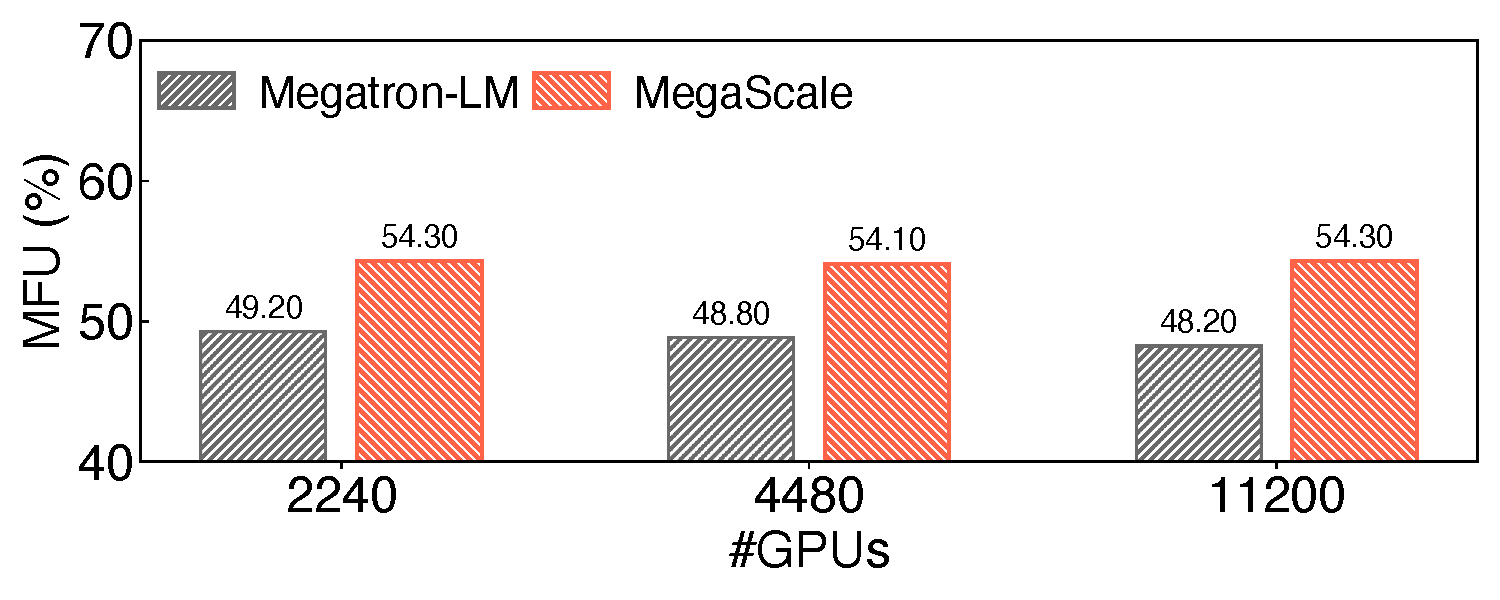
\includegraphics[width=0.46\textwidth]{figures/experience/530B_scaling.pdf}
    \caption{Weak-scaling training performance of Megatron-LM and \sysname on the 530B model, where the batch size is scaled proportionally with the number of GPUs.}
    \label{fig:exp_530b_scaling}
\end{figure}
\parabf{Scalability.} Figure~\ref{fig:exp_530b_scaling} compares Megatron-LM
and {\sysname} when training the 530B model, where we set
the batch size as the number of GPUs with adjusted learning rate to show the MFU results. We see that the MFU of {\sysname} is higher than Megatron-LM
by up to 6.1\%. With increasing scales, the MFU of Megatron-LM decreases by 1.6\%
with more stragglers and communication, while {\sysname} has near-linear
scalability due to 3D-parallel communication overlapping. 

In Table \ref{tab:exp-175b-scaling}, we evaluate the strong-scaling training performance of Megatron-LM and {\sysname} on the 175B model by increasing number of GPUs and maintaining a constant batch size. This experimental setting is more realistic, given that batch size is constrained by convergence effects and cannot be indefinitely scaled with the number of GPUs. {\sysname} achieves up to 1.34$\times$ speedups over Megatron-LM across all settings. With increasing GPUs, we observe the MFU of {\sysname} decreases from 59.1\% to 55.2\%. This is expected since the batch size is fixed and the computation-to-communication ratio decreases with more GPUs. Even in the largest scale with 12,288 GPUs, {\sysname} still outperforms Megatron-LM by 14\% MFU. For the smaller scale training, the speedup of {\sysname} over the baseline ranges from 1.23$\times$ to 1.32$\times$. Note that the difference in the maximum number of GPUs between this and the previous experiments (e.g., 12,288 vs. 11,200) is due to distinct 3D parallelism configurations for 175B and 530B models.


\iffalse
\begin{figure}[!t]
    \centering
   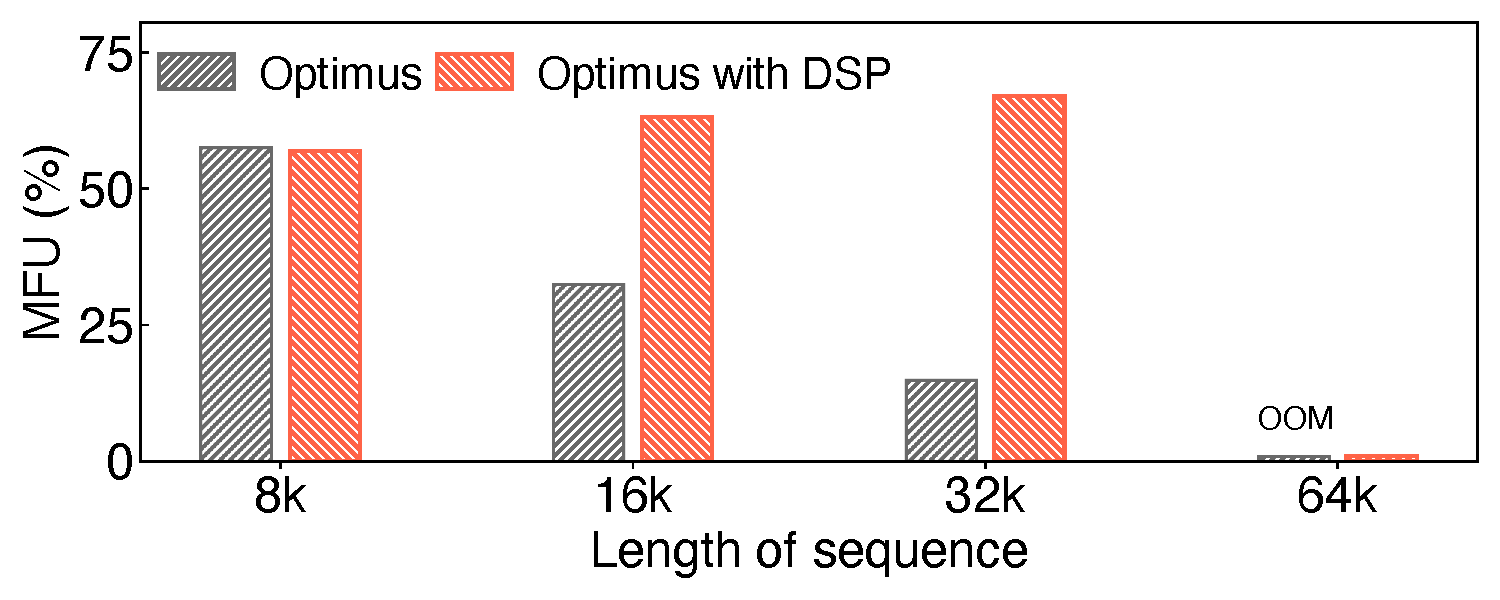
\includegraphics[width=\linewidth]{figures/experience/long_sequence.pdf}
    \vspace{-4mm}
    \caption{Long sequence training. }
    \vspace{1mm}
    \label{fig:exp_long_seq}
\end{figure}
\fi

\iffalse
\begin{figure} [!t]
    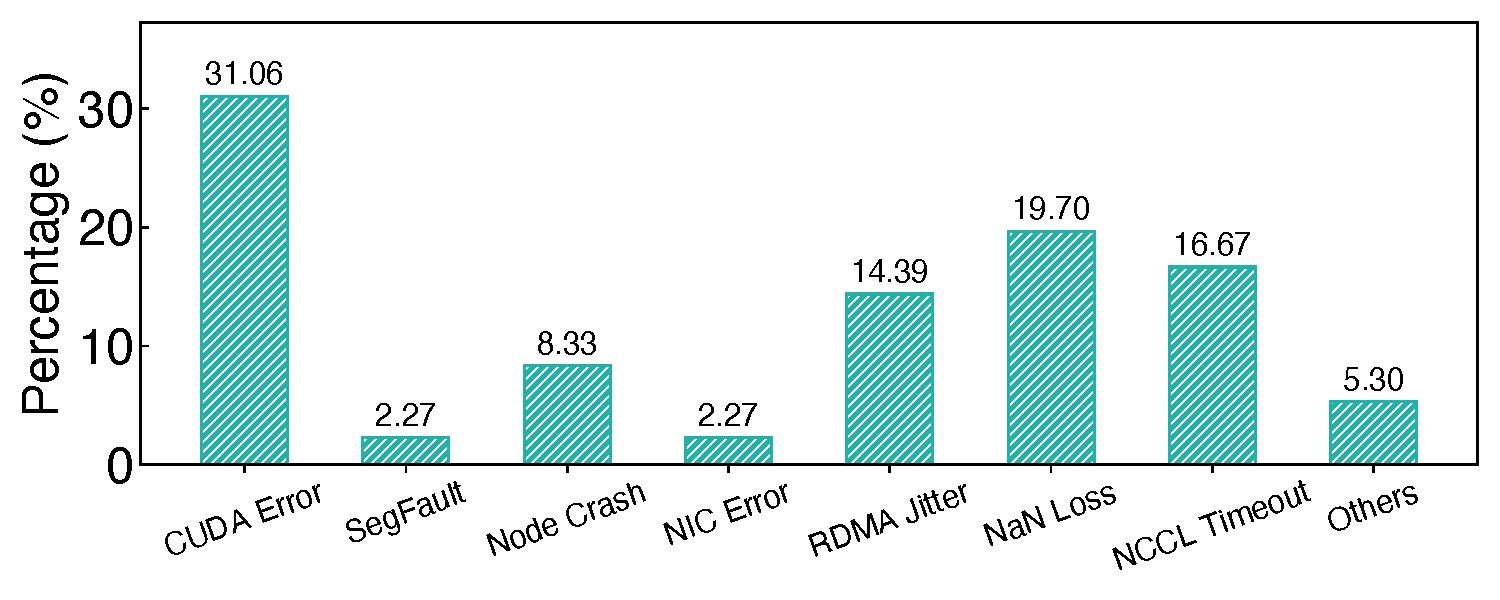
\includegraphics[width=0.45\textwidth]{figures/experience/failure_breakdown.pdf}
    \vspace{-0.15in}
    \caption{Failures breakdown.}
    \label{fig:failure breakdown}
\end{figure}
\fi

\parabf{Ablation study.} 
We evaluate the effectiveness of our optimization techniques of {\sysname}.
Table~\ref{tab:exp-ablation} shows the MFU improvement breakdown with different
optimizations when training the 175B model on 256 GPUs. The baseline \revision{is the original Megatron-LM and} has 47.7\%
MFU. It is worth noting that the networking optimizations are 
turned on for both Megatron-LM and {\sysname} in this evaluation. We first apply 
two algorithmic techniques, parallel transformer block and
sliding window attention, to Megatron-LM, achieving 5.6\% MFU improvement. 
Communication is the major bottleneck of large-scale LLM training, and
the 3D parallel communication overlapping of {\sysname} hides the overhead and
accelerates training by 6.2\% MFU. We further adopt efficient operators and obtain 
1.7\% acceleration. Other optimizations such as data pipeline 
optimizations and the problematic code elimination mentioned 
in \ref{sec:faults_fixed} further achieves 1.1\%
performance gain. Finally, we scale the batch size from 256 to 768 with LAMB
optimizer, which significantly extends the steady phase in interleaved pipeline
parallelism and achieves 3.0\% MFU improvement.  To sum up, {\sysname}
outperforms the baseline by 17.6\% in the MFU number with all these
optimizations.


\begin{table}[t]
    \centering
    \begin{tabular}{|c|c|c|}
        \hline
        Idx & Method & MFU ($\Delta$ MFU) \\
        \hline
        1 &  baseline & 47.7\% \\
        2 &  (1) with PTB & 52.3\% (4.6\%)  \\
        3 &  (2) with SWA & 53.3\% (5.6\%) \\
        4 &  (3) with TP overlap & 55.5\% (7.8\%) \\
        5 &  (4) with PP overlap &  58.0\% (10.3\%)\\
        6 &  (5) with DP overlap &  59.5\% (11.8\%)\\
        7 &  (6) with efficient operators &  61.2\% (13.5\%)\\
        8 &  (7) with misc optimizations & 62.3\% (14.6\%)  \\
        9 & (8) with LAMB (BS$\times$3) &  65.3\% (17.6\%)\\
         \hline
    \end{tabular}
    \caption{MFU improvement breakdown when training the 175B model with 256 GPUs and batch size 256.}
    \label{tab:exp-ablation}
\end{table}

\iffalse
\parabf{Long sequence training.} 
We compare {\sysname} with Megatron-LM on long sequence training tasks with 64 GPUs
on 52B model. With the sequence length increasing from 8k to 64k, we increase
the distributed sequence dimension for {\sysname} while increasing the tensor
parallelism dimension for Megatron-LM to evaluate the performance. As seen in
Figure~\ref{fig:exp_long_seq}, the performance of Megatron-LM decreases
significantly from 8k to 32k as the sequence length increases. When the sequence
length reaches 64k, Megatron-LM encounters out-of-memory (OOM) issue. However,
{\sysname} achieves consistent performance across all settings, which does not
have performance degradation or OOM issue when the sequence length increases. 
\fi


\subsection{Model Convergence and Stability}
\label{sec:experience:covergence}

\begin{figure*}[t]
     \centering
     \begin{subfigure}[b]{0.46\textwidth}
         \centering
         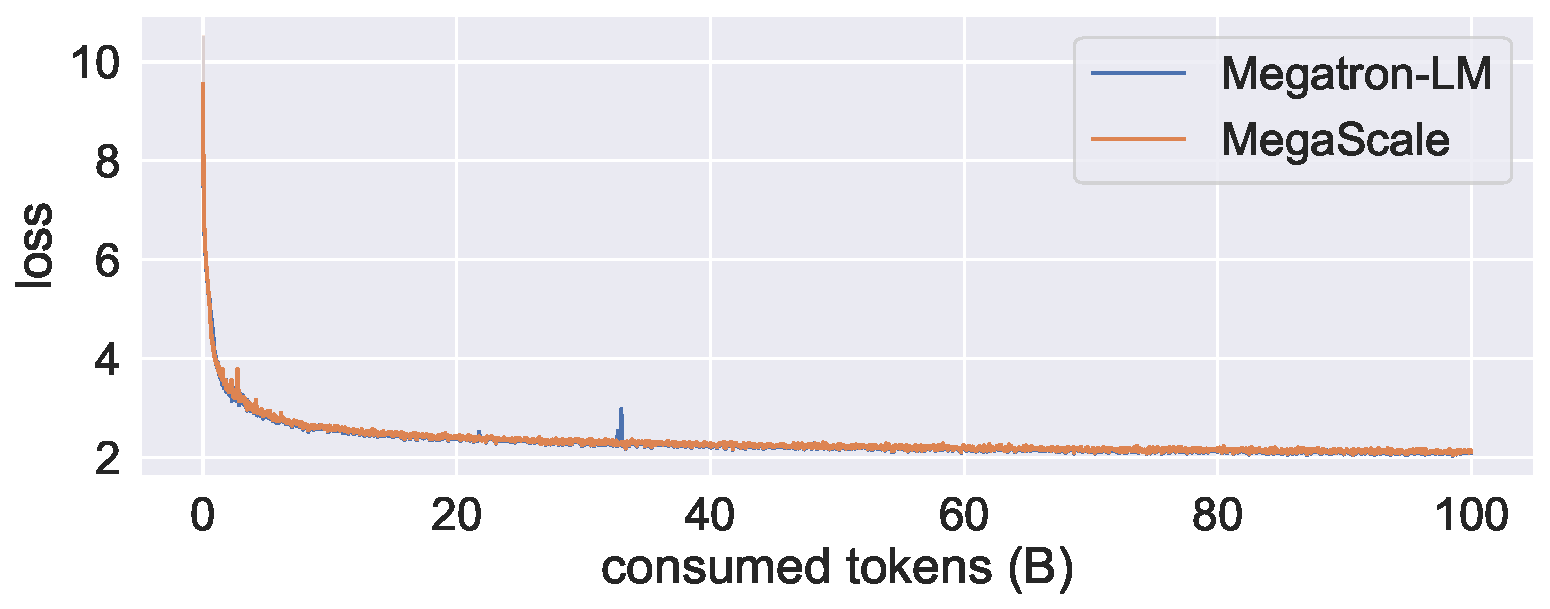
\includegraphics[width=\textwidth]{figures/experience/algo-loss.pdf}
         \caption{The training loss curve of {\sysname}, which includes algorithm optimizations, in comparison with Megatron-LM.}
         \label{fig:algo-loss}
     \end{subfigure}
     \hfill
     \begin{subfigure}[b]{0.46\textwidth}
         \centering
         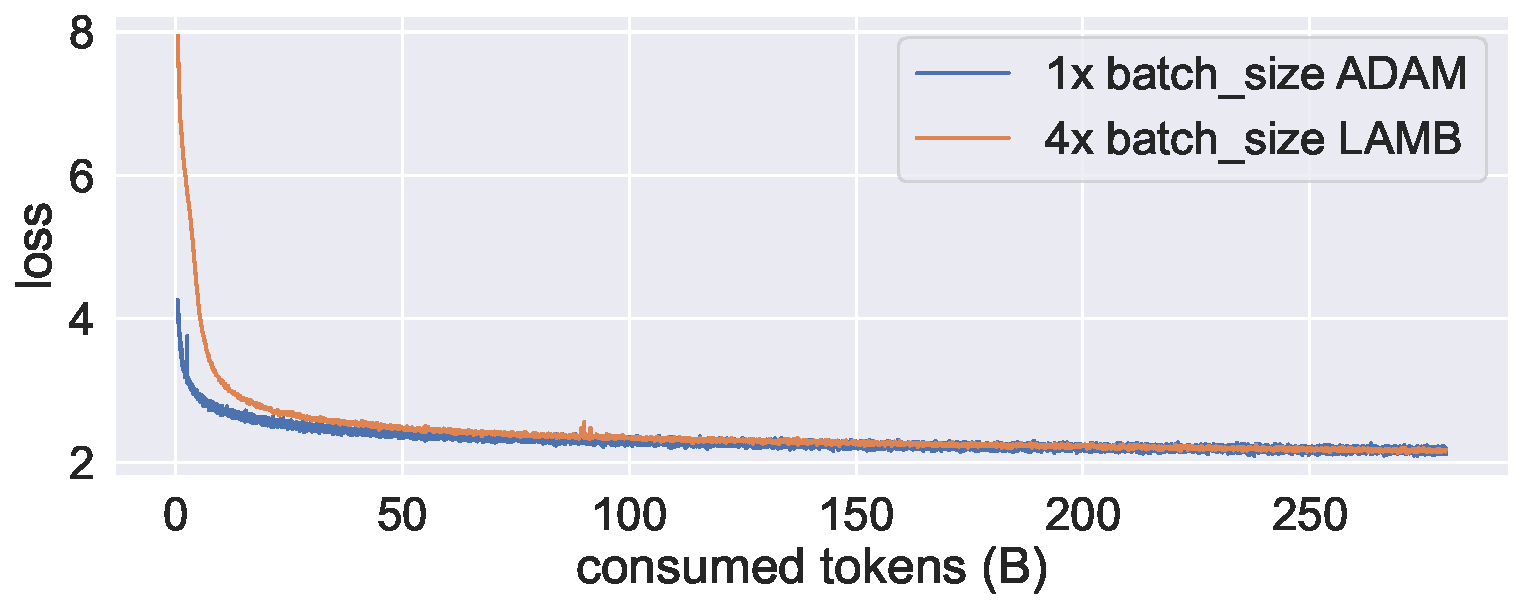
\includegraphics[width=\textwidth]{figures/experience/lamb-loss.pdf}
         \caption{The training loss curve of ADAM optimizer and LAMB optimizer with four times of the batch size.}
         \label{fig:lamb-loss}
     \end{subfigure}
    \caption{The training loss curves in microbenchmark experiments.}
    \label{fig:loss}
\end{figure*}

\begin{figure*}[t]
    \centering
    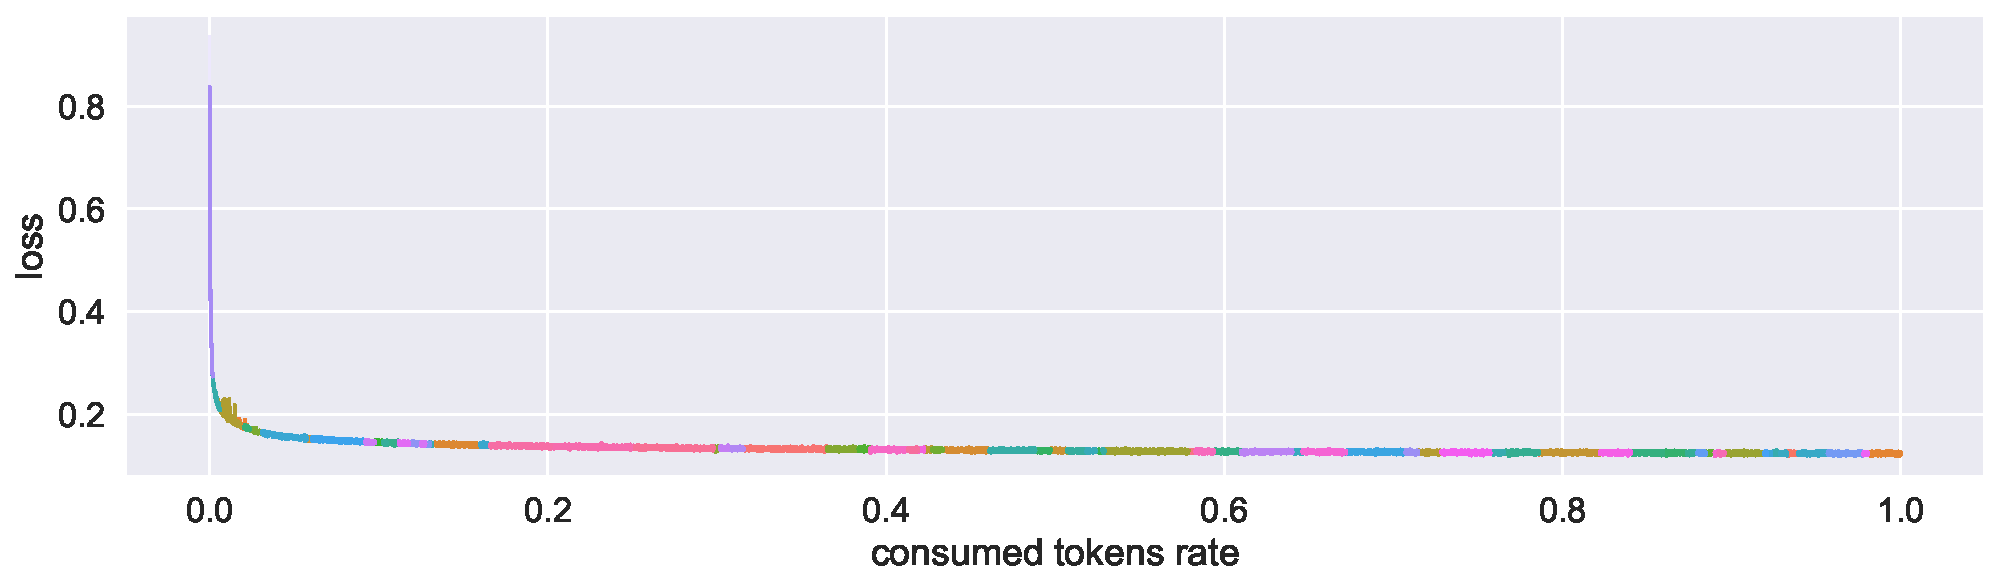
\includegraphics[width=0.95\textwidth]{figures/experience/llm-loss.pdf}
    \caption{The normalized training loss curve of a real production run on more than
    10,000 GPUs for several weeks. This run trains a model with hundreds of
    billions of parameters on multi-trillion tokens. Different colors indicate
    training restarts. \sysname repairs and recovers the training process for
    over 100 times in presence of failures.}
    \label{fig:llm-loss}
\end{figure*}
\paraf{Model convergence microbenchmarks.}
 \revision{We first conduct microbenchmark experiments to validate the algorithm techniques do not affect the model convergence. Due to the resource limit, the microbenchmarks are done on the 13B model.}
As shown in Figure~\ref{fig:algo-loss}, while {\sysname} adopts algorithm techniques, including parallel transformer 
block and sliding window attention, it achieves comparable loss results with 
the baseline when training with more than 100B tokens. We also evaluate the 
effect of LAMB optimizer as depicted in Figure~\ref{fig:lamb-loss}, which shows 
that LAMB optimizer with four times of batch size achieves the same loss as ADAM 
optimizer after around 250B tokens. \revision{Based on these observations, we turn on all the algorithmic optimizations in production training.}


\parabf{Model convergence and stability in real production LLM training.}
We show the model convergence and stability from a real production run. This run
trains a proprietary model with hundreds of billions of parameters on
multi-trillion tokens. This run uses more than 10,000 GPUs and lasts
for several weeks. Figure~\ref{fig:llm-loss} shows the loss continues to
converge, with distinct colors indicating the training is restarted. Over the
several weeks of this run, we experience training restarts over 100 times. With
the robust training framework, over 90\% of software and hardware faults are automatically identified and fixed by the techniques
detailed in~\S\ref{sec:fault_tolerance}. The rest of the problems are handled
with the help of the troubleshooting tools described in~\S\ref{sec:monitor}.

\subsection{Problems Discovered and Fixed}
\label{sec:faults_fixed}

\revision{We conduct an analysis of the fault records for the aforementioned production training job over several weeks. Our findings indicate that over 90\% of the exceptions among them are automatically detected, located, and recovered using our robust training framework, such as CUDA error and segmentation fault. The average time required for detecting failure and executing diagnostic tests is less than 10 minutes. Moreover, the system can catch up to the training progress prior to the crash within 15 minutes from the latest checkpoints, maintaining over 90\% effective training time rate, which is calculated as the number of iterations multiplied by the iteration training time, divided by the total training time. Below we show our experience in diagnosing and fixing some intriguing problems, which need to be analyzed using the troubleshooting tools in~\S\ref{sec:monitor}.}


\parabf{Computational stragglers.} Building upon our utilization of CUDA event timers, we made another pertinent observation across multiple experimental setups. We noted that specific hosts took approximately 10\% more time to execute the same forward computations compared to other ranks. This consistency across different experiments led us to conclude that the issue was not with the software but rather inherent to certain machines in the cluster. After isolating and removing these problematic hosts from the cluster, we observed an approximate 0.7\% improvement in MFU.

\begin{figure}
    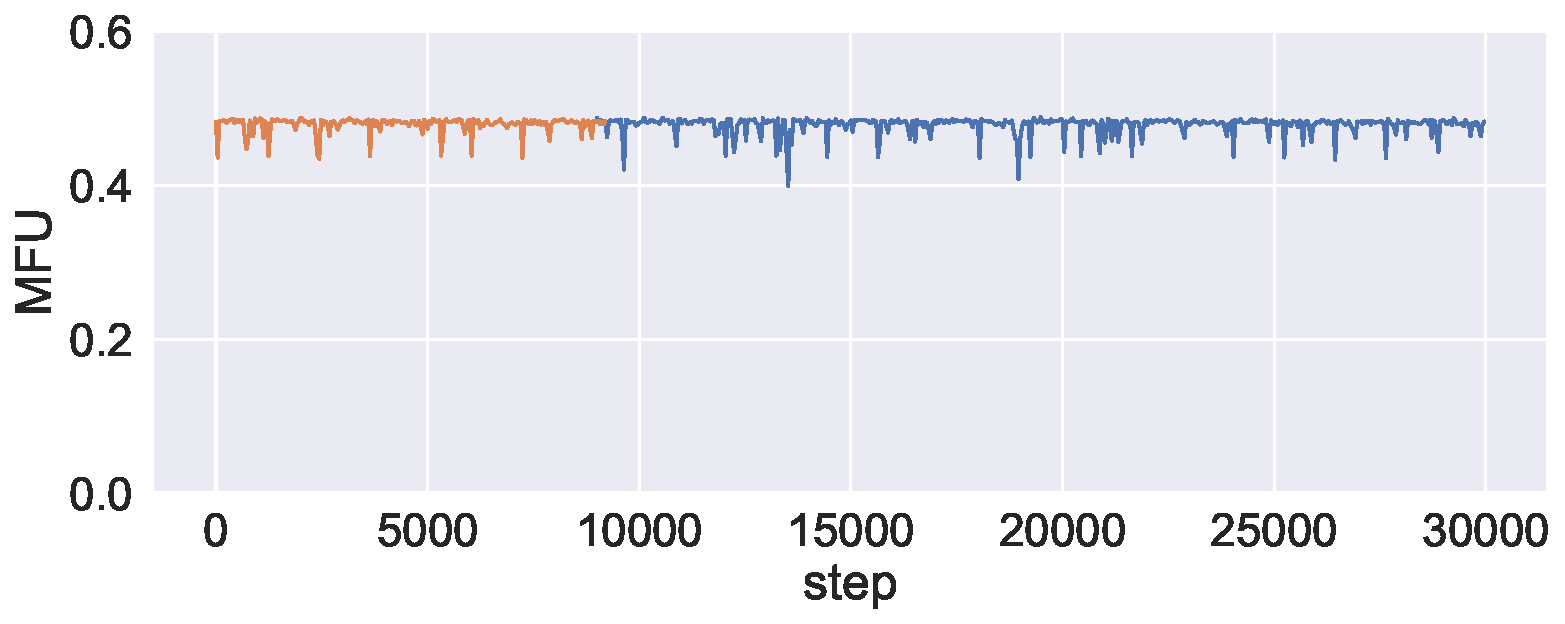
\includegraphics[width=0.46\textwidth]{figures/experience/mfu-stable.pdf}
    \caption{The MFU becomes stable after addressing the stragglers and problematic code segments. \revision{Different colors represent different training trials with the same setup.}}
    \label{fig:mfu-stable}
\end{figure}

\parabf{MFU decreasing.} In such large-scale training experiments, another phenomenon we observed is that training efficiency did not remain consistent over time. Instead, as the training progressed, the MFU of our training job gradually decreased. Through a step-by-step analysis based on CUDA event timer metrics, we noted several key findings. While the time consumed per training step was increasing, the time spent on forward, backward, and optimizer computations remained stable, irrespective of the increasing number of steps. This led us to infer that the time increase must be attributed to the collective communication overhead. Upon a reverse chronological examination, we identified the last collective communication step as the gradient reduce-scatter in data parallelism. If this step is delayed, the overall time per step elongates. Since we observed network bandwidth to be largely stable, we ruled out slowed communication speed as a factor for the increased time. According to the synchronization characteristics of collective communication, this leaves us with one conclusion: some ranks initiate the reduce-scatter operation later than others, forcing a wait for the slowest rank to catch up. In a scaled-down experiment involving only two ranks per data parallel group, we measured the launch times for reduce-scatter calls and found them to not be consistently staggered but rather fluctuating reciprocally. Furthermore, the size of this time stagger increased as more steps were executed. Specifically, Rank A may initially lag behind Rank B but might eventually surpass Rank B in speed and by a growing margin. Ultimately, all ranks waited for the slowest rank. To trace back the root cause of this time skew, we located the variance to occur during the forward computation stage. Digging deeper into the code, we attributed this irregularity to fluctuations caused by 
some code segments. \revision{For instance, irregular garbage collection can introduce disturbances into the training procedure, and certain PyTorch operations can lead to performance fluctuations. } These operations are on the critical path but can be affected along the training procedure. After modifying or removing those problematic code segments, we no longer observed a significant decline in MFU, as shown in Figure~\ref{fig:mfu-stable}.



\parabf{Frequent network interface flapping problem.} We occasionally encounter training stall or training speed drop problem due to frequent network interface flapping. When the network interface flapping phenomena happens, the network interface goes down at first then goes up again. The interval between down and up time usually lasts for several seconds. During the down process, all the packets in transmission will be dropped. The first lesson we learn is the timeout threshold should be set explicitly to a larger value , otherwise the default value will make NCCL timeout very quickly and return a completion error before the network card up again. The second lesson we learn is that the root cause of this problem is the bad link quality between network card, AOC cable and switch. The flapping frequency can be reduced to a satisfactory level by doing lower level quality control over network card signal strength, AOC cable quality and switch side signal strength. 
